\documentclass[10pt, journal,compsoc]{article}
\usepackage{graphicx}
\usepackage{latexsym}
\usepackage{amsfonts}
\usepackage{listings}
\usepackage{mypriptrt} 

\begin{document}

\title{Neural Computation LU - Aufgabenblock 1 - Gruppe 8}


\author{Aitor Aldomà \and Thomas Kern \and Christian Weichselbaum}
        

\section{Exercise 1.1}
\subsection{Exercise 1.1.1}
\textit{Stellen Sie die Lage der Datenvektoren und ihre labels graphisch dar.}

\begin{figure}[htp]
	\centering
	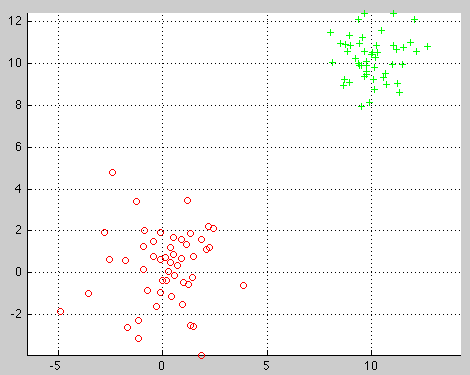
\includegraphics[width=1\textwidth]{ab1_1_1}
	\caption{Datensatz generiert mit genData(50,2)}\label{fig:1}
\end{figure}

\subsection{Exercise 1.1.2}

\textit{Untersuchen sie den Trainingsalgorithmus: Wieviele Iterationen werden benötigt, bis sich weight-Vektor $w$ im Fall von linear separierbaren Daten nicht mehr andert?}
\\
It takes 9 epochs until the weight vector doesn't change. At this point, the algorithm stops because all of the data entries are successfully classified.
\\
\\
\textit{Wie verändert sich der w während des Trainings?}
\\
The weight vector is changed at each iteration IFF the data entry is misclassified. If it is misclassified the product of gamma, data entry and target for the data entry is added to the current weight vector.
\\
\\

\textit{Welchen Einfluss hat die Schrittweite?}
\\
Gamma has a huge impact on the weight vector and number of epochs required to successfully classify all the entries. In our randomly generated dataset (1.1.1), changing gamma from 0.1 to 0.3 resulted in 7 epochs instead of 9 epochs (win of 22\%) as well as a value-bloated weight vector (end weight vector:  [5.2000 0.5503 -2.1547] instead of [5.2000 0.5503 -2.1547]).
\\
\\

\textit{Plotten Sie die Daten und Entscheidungsgrenze in $R^2$}
\\
TODO TODO TODO TODO TODO TODO TODO TODO TODO TODO TODO TODO
\\
\\

\textit{Wie ist das Verhalten bei nicht linear separierbaren Daten?}
\\
Unfortunately, the algorithm runs until maxIts (variable setting the maximum of possible epochs) is reached. Since the data is not linearly seperable there will always be a data entry on the wrong side of the hyperplane and therefor rotating it will not result in a success. The algorithm would run indefinitely without maxIts. 

\subsection{Exercise 1.1.3}

\section{Exercise 1.2}
\subsection{Exercise 1.2.1}
asdf
\end{document}


